\chapter{Experiments}
\label{chapter:experiments}


\section{Full Lap Planning Test}

In this experiment we will test the Hybrid A* and \gls{SEHS} algorithms as we described them in Section~\ref{sec:trajectory_planning_algorithms} on several different circuit maps. For each circuit, their task will be to find a near time-optimal trajectory from a starting position through a series of waypoints until the last waypoint of the circuit is reached. We will then compare the quality of the solutions, how much of the state space the algorithm had to explore before it found the solution, and how long it took to calculate the result.

\subsection{Test Setup}

The parameters of the vehicle chassis and the vehicle model we used are equal to the properties of our experimental vehicle as stated in Table~\ref{table:dimensions} and derived in Section~\ref{sec:actuators_model}.

Both Hybrid A* and \gls*{SEHS} require specification of state space and time discretization parameters. We found that both algorithms performed well with time step $\Delta t=\SI{0.04}{\second}$ (\SI{25}{\hertz}), the heading angle values divided into \num{24} sectors of a circle, and the range of possible values of motor \gls*{RPM} divided into \num{50} sub-ranges. Additionally, the Hybrid A* algorithm splits the $x$ and $y$ coordinates were split into squares with side lengths of $4r$, where $r$ is the radius of the vehicle. The SEHS algorithm discretizes the $xy$ plane by finding a path of circles in the Space Exploration step. We require the radii of the circles to be between $r$ a $4r$

The actions available to the planner were a cross product of 5 throttle levels (\num{-1}, \num{0}, \num{0.33}, \num{0.66}, \num{1}) and 5 target steering angles (\num{-1}, \num{-0.5}, \num{0}, \num{0.5}, \num{1}). This limits the possible maneuvers of the vehicle, but it allows the planner to run reasonably fast.

For each circuit, we first perform track segmentation, as described in Section~\ref{sec:track_segmentation}, to detect corners which we use as waypoints. We also perform the Space Exploration step of the SEHS algorithm. We then let both algorithms find the near time-optimal trajectory from the initial configuration defined for each circuit to the last waypoint. We measure the number of search nodes the algorithm opens during search, the number of search nodes which are expanded, and also the time it takes to find the solution on a testing computer. Because both of the algorithms are deterministic, they always find the same solution for the same problem and they always open and expand the same number of search nodes. The execution times differ slightly and so we repeat the measurement 100 times and calculate the mean execution time.

The computer we used for measurement uses an Intel Core i5-7200U CPU running at the base clock of \SI{2.71}{\giga\hertz} and 16 GB of DDR4 RAM at the base clock of \SI{2133}{\mega\hertz}. The source code was written in C++ and compiled using GCC 9.2 with the \texttt{-O3} optimization flag.

\subsection{Results}

\begin{figure}[!tbp]%
	\centering

	\begin{subfigure}[t]{\textwidth}
		\begin{subfigure}[t]{0.45\textwidth}
			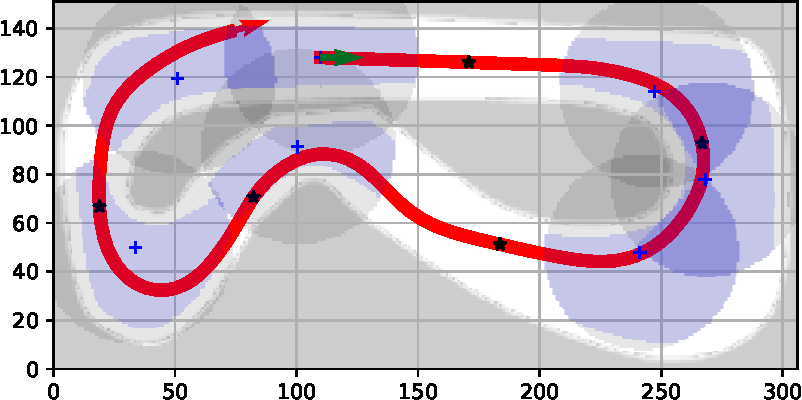
\includegraphics[width=\textwidth]{../img/experiments/porto-hybrid_astar-trajectory}
		\end{subfigure}
		\hfill
		\begin{subfigure}[t]{0.45\textwidth}
			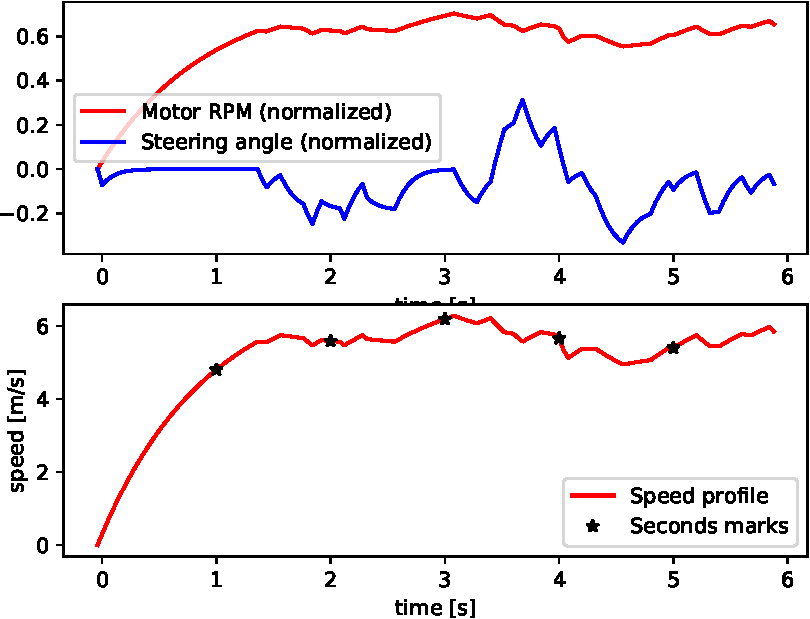
\includegraphics[width=\textwidth]{../img/experiments/porto-hybrid_astar-actuators}
		\end{subfigure}
		\caption{Solution found by Hybrid A*}
		\label{fig:solution_porto-hybrid_astar}	
	\end{subfigure}
	
	\vspace{0.75cm}
	
	\begin{subfigure}[t]{\textwidth}
		\begin{subfigure}[t]{0.45\textwidth}
			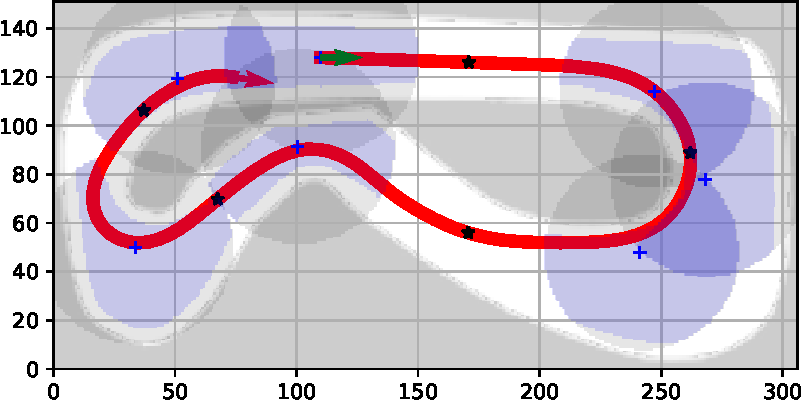
\includegraphics[width=\textwidth]{../img/experiments/porto-sehs-trajectory}
		\end{subfigure}
		\hfill
		\begin{subfigure}[t]{0.45\textwidth}
			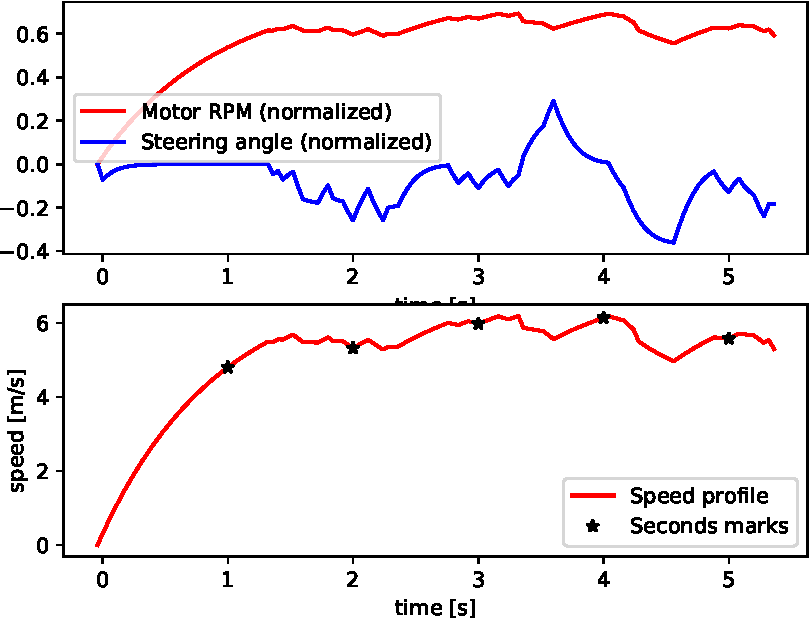
\includegraphics[width=\textwidth]{../img/experiments/porto-sehs-actuators}
		\end{subfigure}
		\caption{Solution found by SEHS}
		\label{fig:solution_porto-sehs}
	\end{subfigure}

	\vspace{0.75cm}
	
	\begin{subfigure}[t]{\textwidth}
		\centering
		\begin{tabular}{l r r r r r}%
			\toprule
			Algorithm & Opened & Expanded & Search time & Distance & Lap time \\
			\midrule
			Hybrid A* & \num{102430} & \num{11957} & \SI{166.55}{\milli\second} & \SI{30.39}{\meter} & \SI{5.92}{\second} \\
			SEHS & \bftab \num{93936} & \bftab \num{11070} & \bftab \SI{165.30}{\milli\second} & \bftab \SI{26.88}{\meter} & \bftab \SI{5.40}{\second} \\
			\bottomrule
		\end{tabular}
		\caption{Comparison of the solutions and computation requirements.}
		\label{table:porto}
	\end{subfigure}

	\vspace{0.75cm}
	
	\caption{Track ``Porto''}
\end{figure}


\begin{figure}[!tbp]%
	\centering
	
	\begin{subfigure}[t]{\textwidth}
		\begin{subfigure}[t]{0.45\textwidth}
			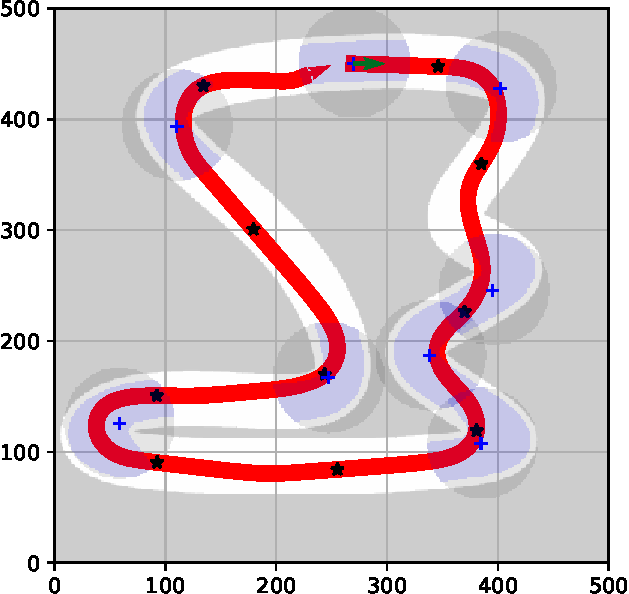
\includegraphics[width=\textwidth]{../img/experiments/tornado-hybrid_astar-trajectory}
		\end{subfigure}
		\hfill
		\begin{subfigure}[t]{0.45\textwidth}
			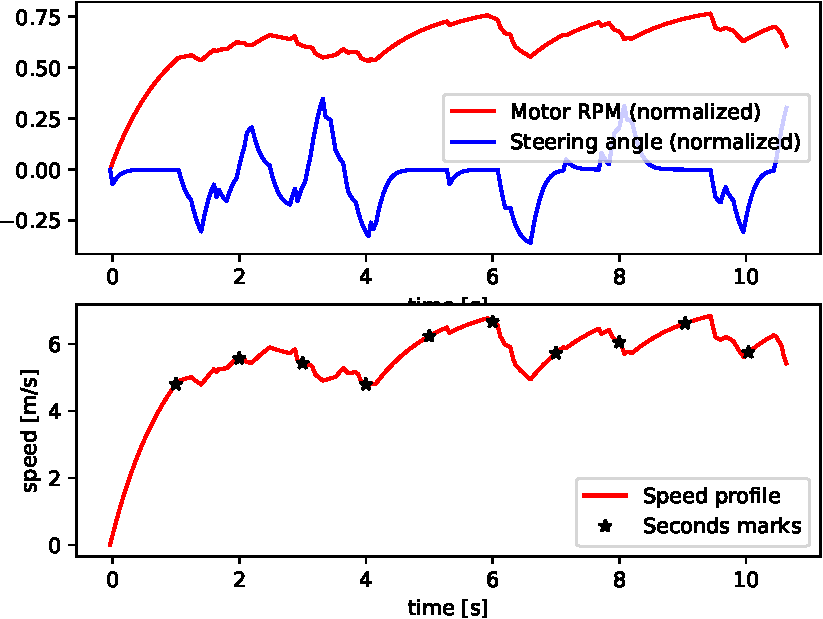
\includegraphics[width=\textwidth]{../img/experiments/tornado-hybrid_astar-actuators}
		\end{subfigure}
		\caption{Solution found by Hybrid A*}
		\label{fig:solution_tornado-hybrid_astar}	
	\end{subfigure}
	
	\vspace{0.75cm}
	
	\begin{subfigure}[t]{\textwidth}
		\begin{subfigure}[t]{0.45\textwidth}
			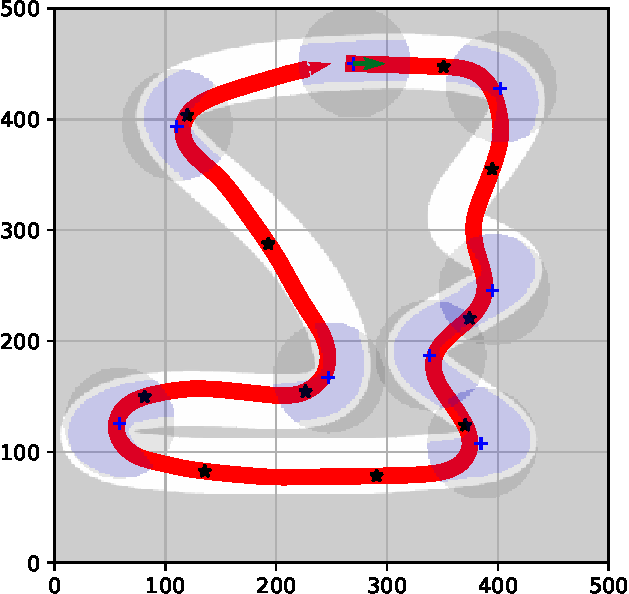
\includegraphics[width=\textwidth]{../img/experiments/tornado-sehs-trajectory}
		\end{subfigure}
		\hfill
		\begin{subfigure}[t]{0.45\textwidth}
			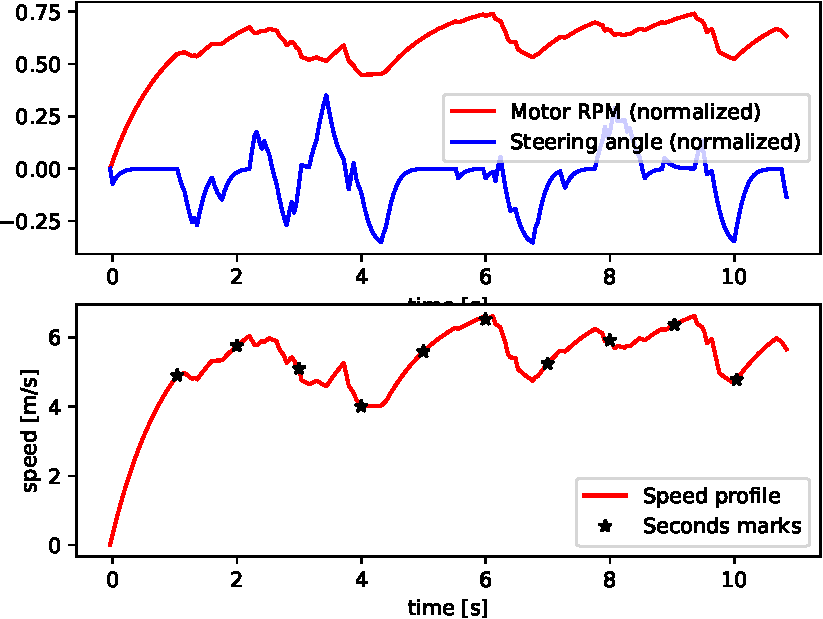
\includegraphics[width=\textwidth]{../img/experiments/tornado-sehs-actuators}
		\end{subfigure}
		\caption{Solution found by SEHS}
		\label{fig:solution_tornado-sehs}
	\end{subfigure}
	
	\vspace{0.75cm}
	
	\begin{subfigure}[t]{\textwidth}
		\centering
		\begin{tabular}{l r r r r r}%
			\toprule
			Algorithm & Opened & Expanded & Search time & Distance & Lap time \\
			\midrule
			Hybrid A* & \num{184864} & \num{21874} & \SI{322.95}{\milli\second} & \SI{59.0759}{\meter} & \bftab \SI{10.68}{\second} \\
			SEHS & \bftab \num{129022} & \bftab \num{15232} & \bftab \SI{257.95}{\milli\second} & \bftab \SI{57.7269}{\meter} & \SI{10.80}{\second} \\
			\bottomrule
		\end{tabular}
		\caption{Comparison of the solutions and computation requirements.}
		\label{table:tornado}
	\end{subfigure}
	
	\vspace{0.75cm}
	
	\caption{Track ``Tornado''}
\end{figure}

\begin{figure}[!tbp]%
	\centering

	\begin{subfigure}[t]{\textwidth}
		\begin{subfigure}[t]{0.45\textwidth}
			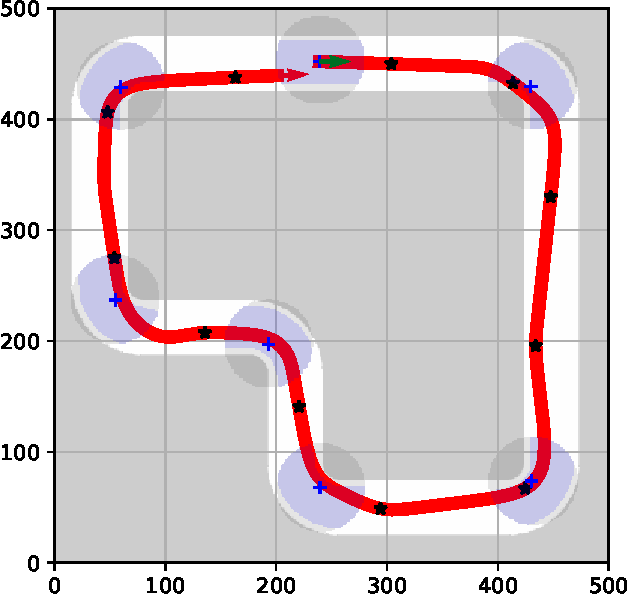
\includegraphics[width=\textwidth]{../img/experiments/simple-hybrid_astar-trajectory}
		\end{subfigure}
		\hfill
		\begin{subfigure}[t]{0.45\textwidth}
			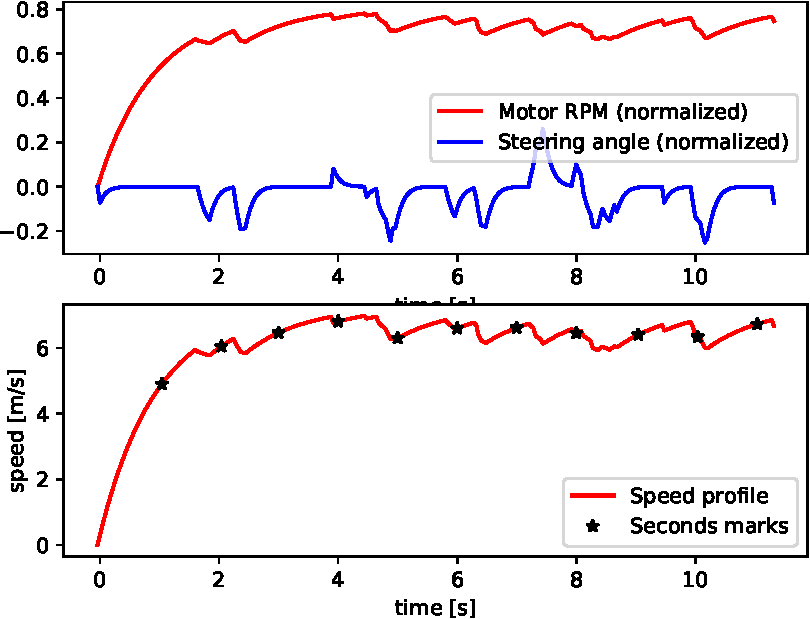
\includegraphics[width=\textwidth]{../img/experiments/simple-hybrid_astar-actuators}
		\end{subfigure}
		\caption{Solution found by Hybrid A*}
		\label{fig:simple-hybrid_astar}
	\end{subfigure}

	\vspace{0.75cm}
	
	\begin{subfigure}[t]{\textwidth}
		\begin{subfigure}[t]{0.45\textwidth}
			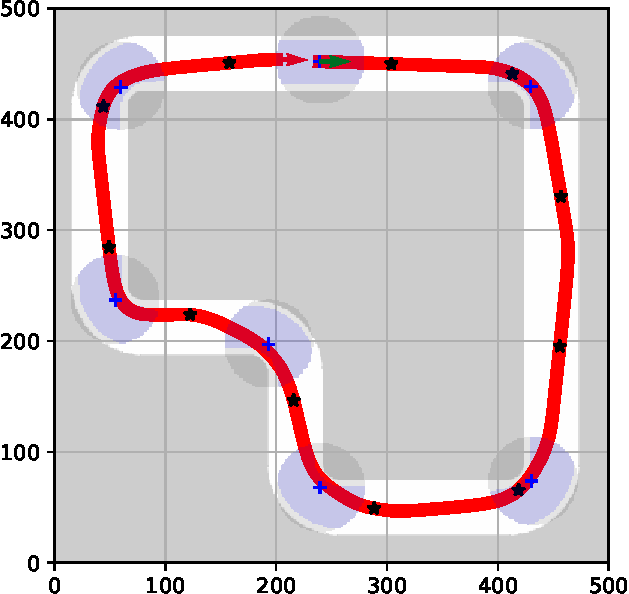
\includegraphics[width=\textwidth]{../img/experiments/simple-sehs-trajectory}
		\end{subfigure}
		\hfill
		\begin{subfigure}[t]{0.45\textwidth}
			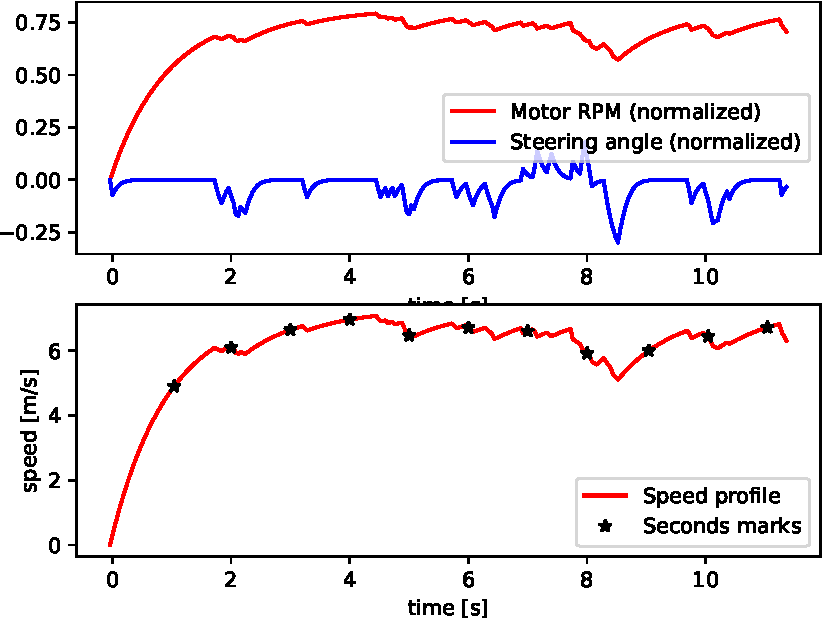
\includegraphics[width=\textwidth]{../img/experiments/simple-sehs-actuators}
		\end{subfigure}
		\caption{Soultion found by SEHS}
		\label{fig:simple-sehs}
	\end{subfigure}

	\vspace{0.75cm}

	\begin{subfigure}[t]{\textwidth}
		\centering
		\begin{tabular}{l r r r r r}%
			\toprule
			Algorithm & Opened & Expanded & Search time & Distance & Lap time \\
			\midrule
			Hybrid A* & \num{324109} & \num{37123} & \SI{549.33}{\milli\second} & \bftab \SI{69.18}{\meter} & \bftab \SI{11.36}{\second} \\
			SEHS & \bftab \num{193095} & \bftab \num{22003} & \bftab \SI{372.49}{\milli\second} & \SI{69.60}{\meter} & \bftab \SI{11.36}{\second} \\
			\bottomrule
		\end{tabular}
		\caption{Comparison of the solutions and computation requirements.}
		\label{table:simple}
	\end{subfigure}
	
	\vspace{0.75cm}

	\caption{Track ``Simple''}
\end{figure}

\begin{figure}[!tbp]%
	\centering
	\begin{subfigure}[t]{\textwidth}
		\begin{subfigure}[t]{0.45\textwidth}
			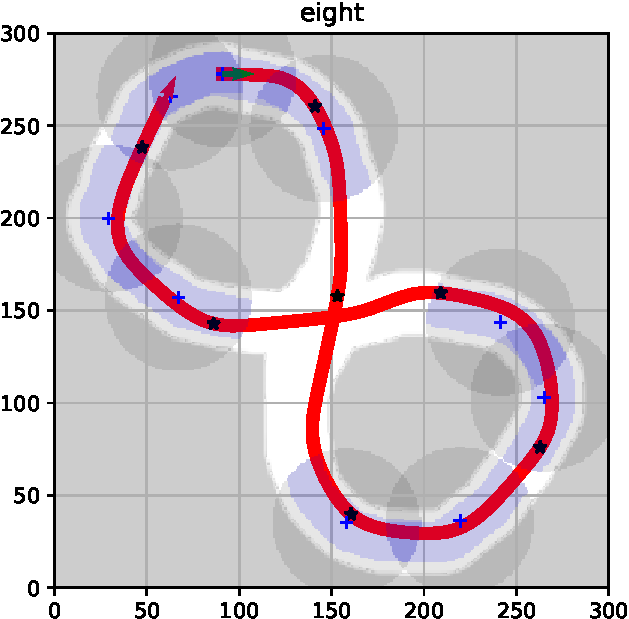
\includegraphics[width=\textwidth]{../img/experiments/eight-hybrid_astar-trajectory}
		\end{subfigure}
		\hfill
		\begin{subfigure}[t]{0.45\textwidth}
			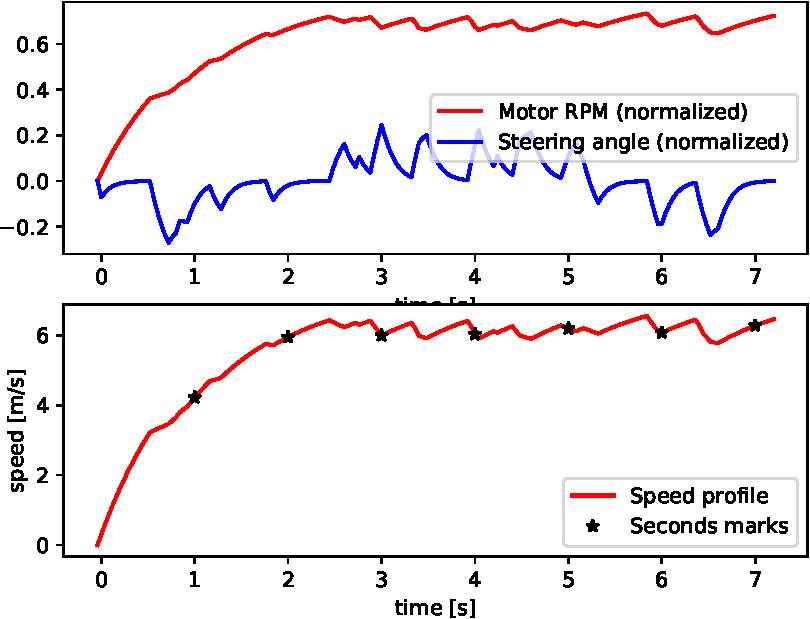
\includegraphics[width=\textwidth]{../img/experiments/eight-hybrid_astar-actuators}
		\end{subfigure}
		\caption{Solution found by Hybrid A*}
		\label{fig:eight-hybrid_astar}
	\end{subfigure}
	
	\vspace{0.75cm}
	
	\begin{subfigure}[t]{\textwidth}
		\begin{subfigure}[t]{0.45\textwidth}
			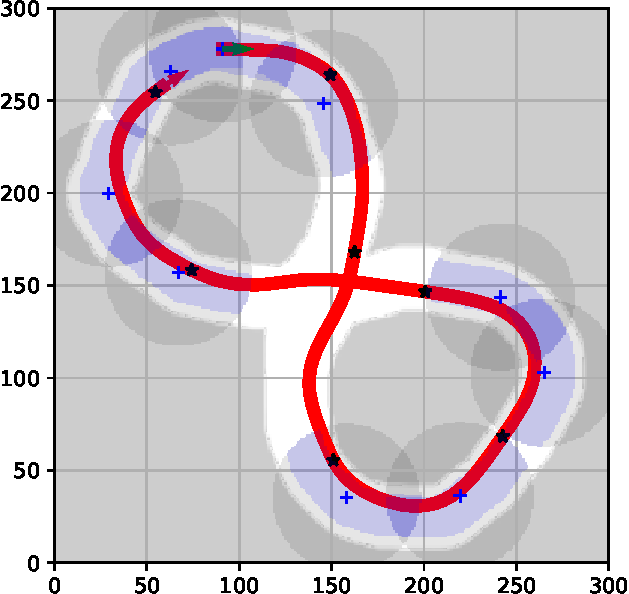
\includegraphics[width=\textwidth]{../img/experiments/eight-sehs-trajectory}
		\end{subfigure}
		\hfill
		\begin{subfigure}[t]{0.45\textwidth}
			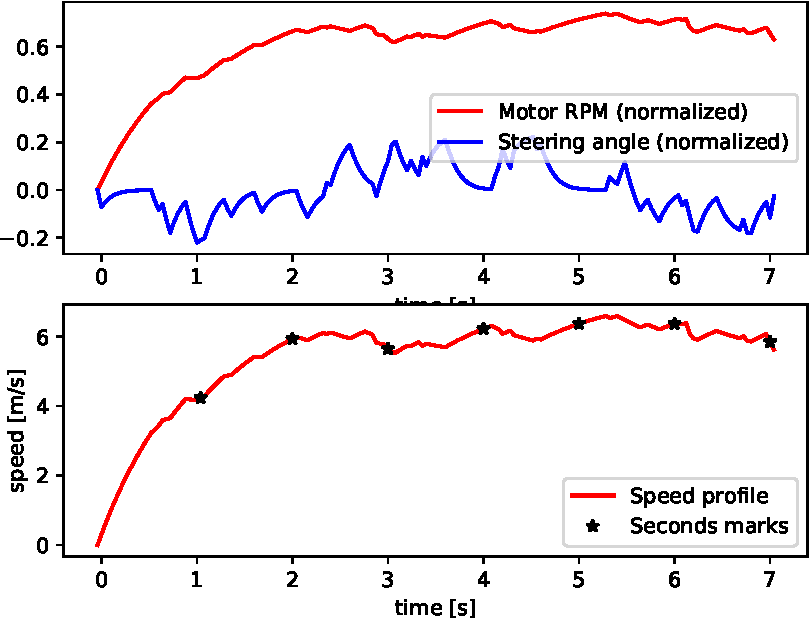
\includegraphics[width=\textwidth]{../img/experiments/eight-sehs-actuators}
		\end{subfigure}
		\caption{Solution found by SEHS}
		\label{fig:eight-sehs}
	\end{subfigure}
	
	\vspace{0.75cm}
	
	\begin{subfigure}[t]{\textwidth}
		\centering
		\begin{tabular}{l r r r r r}%
			\toprule
			Algorithm & Opened & Expanded & Search time & Distance & Lap time \\
			\midrule
			Hybrid A* & \bftab \num{188160} & \bftab \num{22173} & \bftab \SI{328.57}{\milli\second} & \SI{40.26}{\meter} & \SI{7.24}{\second} \\
			SEHS & \num{298325} & \num{36008} & \SI{563.19}{\milli\second} & \bftab \SI{37.77}{\meter} & \bftab \SI{6.88}{\second} \\
			\bottomrule
		\end{tabular}
		\caption{Comparison of the solutions and computation requirements.}
		\label{table:eight}
	\end{subfigure}
	
	\vspace{0.75cm}
	
	\caption{Track ``Eight''}
\end{figure}

\begin{figure}[!tbp]%
	\centering

	\begin{subfigure}[t]{\textwidth}
		\begin{subfigure}[t]{0.45\textwidth}
			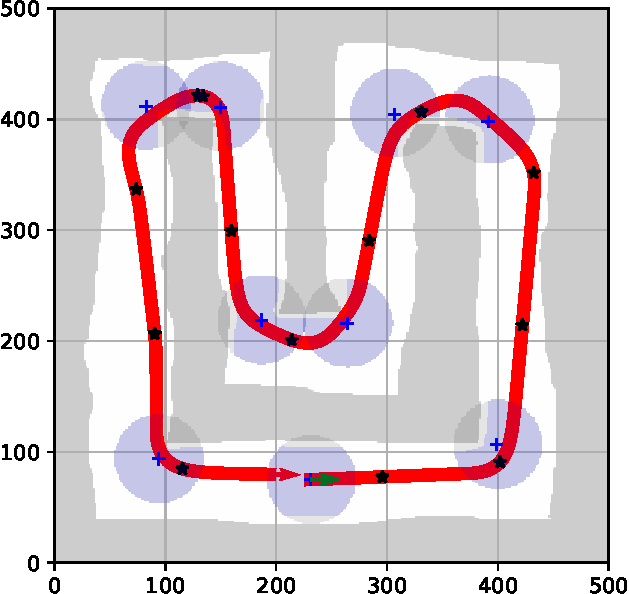
\includegraphics[width=\textwidth]{../img/experiments/u-hybrid_astar-trajectory}
		\end{subfigure}
		\hfill
		\begin{subfigure}[t]{0.45\textwidth}
			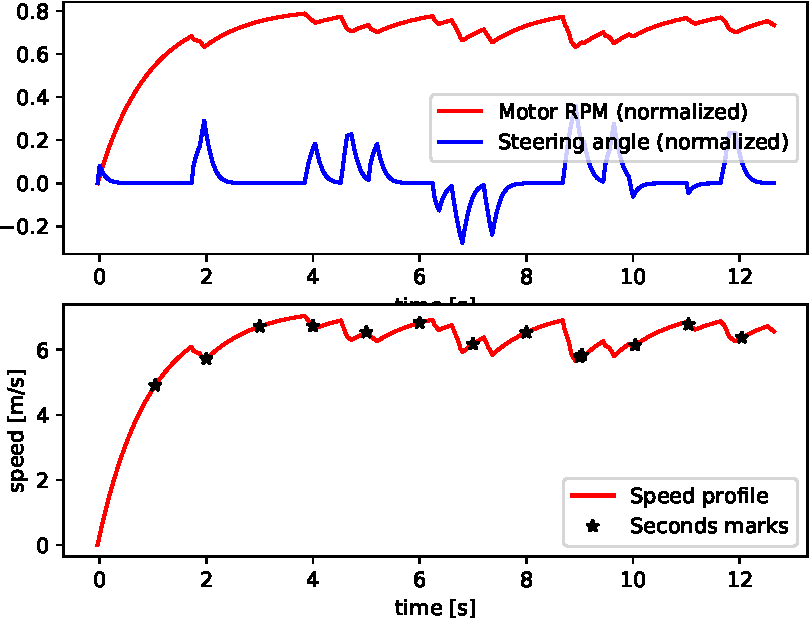
\includegraphics[width=\textwidth]{../img/experiments/u-hybrid_astar-actuators}
		\end{subfigure}	
		\caption{Solution found by Hybrid A*}
		\label{fig:u-hybrid_astar}
	\end{subfigure}

	\vspace{0.75cm}

	\begin{subfigure}[t]{\textwidth}
		\begin{subfigure}[t]{0.45\textwidth}
			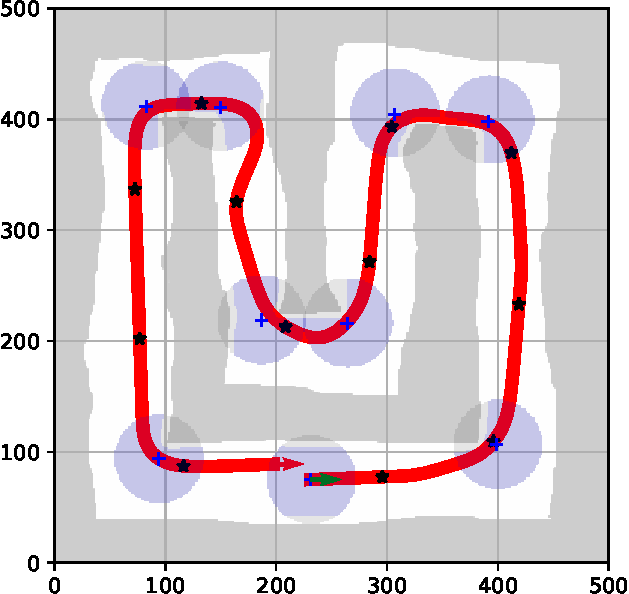
\includegraphics[width=\textwidth]{../img/experiments/u-sehs-trajectory}
		\end{subfigure}
		\hfill
		\begin{subfigure}[t]{0.45\textwidth}
			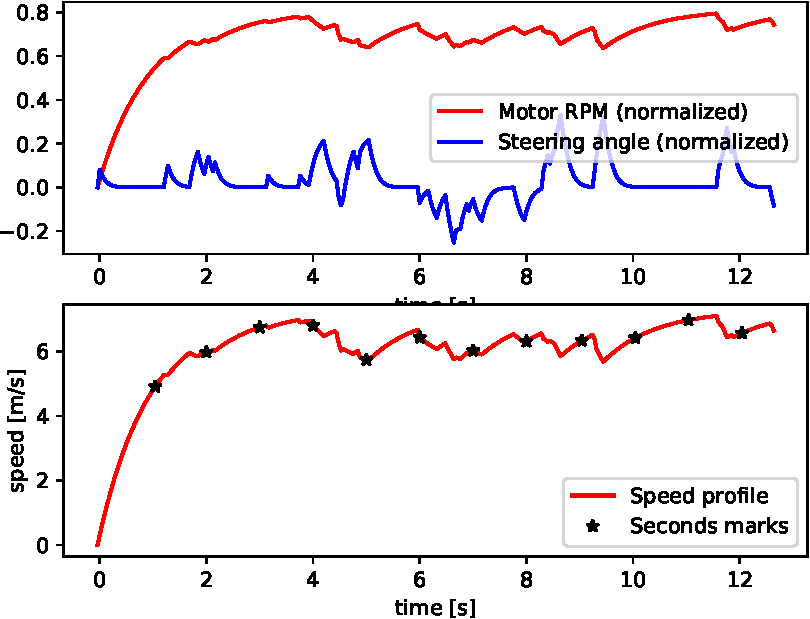
\includegraphics[width=\textwidth]{../img/experiments/u-sehs-actuators}
		\end{subfigure}
		\caption{Solution found by SEHS}
		\label{fig:u-sehs}
	\end{subfigure}
	
	\vspace{0.75cm}
	
	\begin{subfigure}[t]{\textwidth}
		\centering
		\begin{tabular}{l r r r r r}%
		\toprule
		Algorithm & Opened & Expanded & Search time & Distance & Lap time \\
		\midrule
		Hybrid A* & \num{20297799} & \num{2472203} & \SI{64290.3}{\milli\second} & \SI{77.79}{\meter} & \SI{12.68}{\second} \\
		SEHS & \bftab \num{4949842} & \bftab \num{590288} & \bftab \SI{14058.7}{\milli\second} & \bftab \SI{75.91}{\meter} & \bftab \SI{12.56}{\second} \\
		\bottomrule
	\end{tabular}
	\caption{Comparison of the solutions and computation requirements.}
	\label{table:u}
	\end{subfigure}
	
	\vspace{0.75cm}
	
	\caption{Track ``U''}
\end{figure}

\begin{figure}[!tbp]%
	\centering
		
	\begin{subfigure}[t]{\textwidth}
		\begin{subfigure}[t]{0.45\textwidth}
			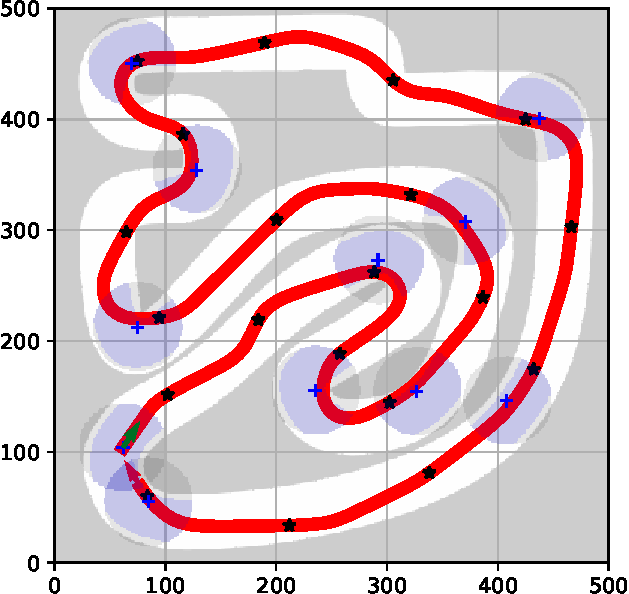
\includegraphics[width=\textwidth]{../img/experiments/zurich-hybrid_astar-trajectory}
		\end{subfigure}
		\hfill
		\begin{subfigure}[t]{0.45\textwidth}
			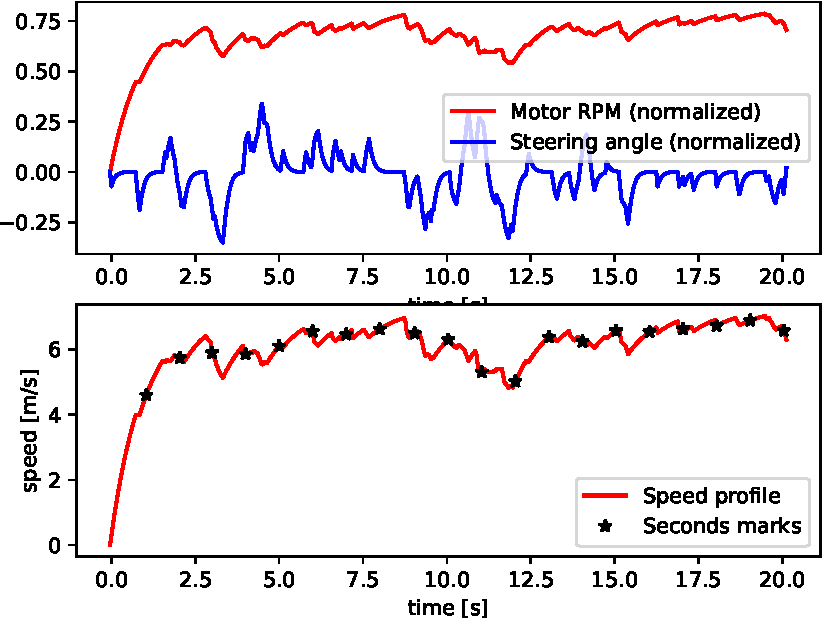
\includegraphics[width=\textwidth]{../img/experiments/zurich-hybrid_astar-actuators}
		\end{subfigure}
		\caption{Solution found by Hybrid A*}
		\label{fig:zurich-hybrid_astar}
	\end{subfigure}

	\vspace{0.75cm}
	
	\begin{subfigure}[t]{\textwidth}	
		\begin{subfigure}[t]{0.45\textwidth}
			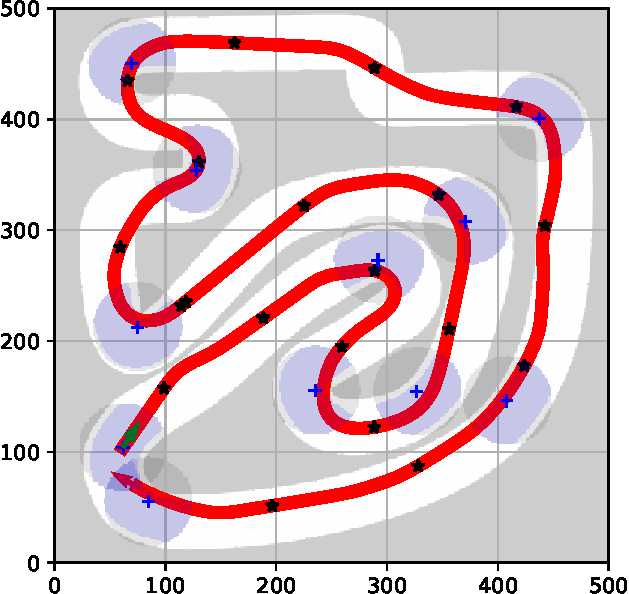
\includegraphics[width=\textwidth]{../img/experiments/zurich-sehs-trajectory}
		\end{subfigure}
		\hfill
		\begin{subfigure}[t]{0.45\textwidth}
			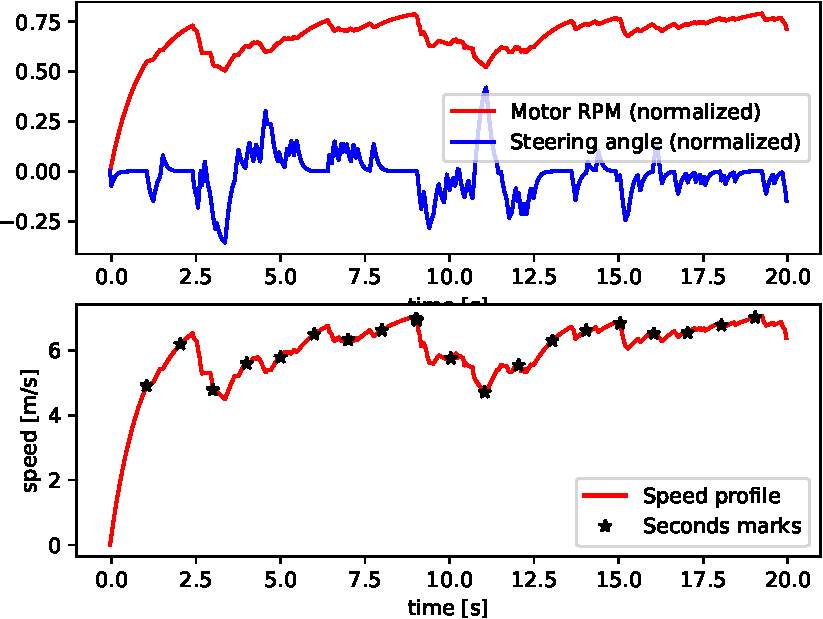
\includegraphics[width=\textwidth]{../img/experiments/zurich-sehs-actuators}
		\end{subfigure}
		\caption{Solution found by SEHS}
		\label{fig:zurich-sehs}
	\end{subfigure}

	\vspace{0.75cm}
	
	\begin{subfigure}[t]{\textwidth}
		\centering
		\begin{tabular}{l r r r r r}%
			\toprule
			Algorithm & Opened & Expanded & Search time & Distance & Lap time \\
			\midrule
			Hybrid A* & \num{5934391} & \num{715557} & \SI{13579.90}{\milli\second} & \textbf{\SI{121.58}{\meter}} & \textbf{\SI{20.16}{\second}} \\
			SEHS & \textbf{\num{1585340}} & \textbf{\num{590288}} & \textbf{\SI{4078.63}{\milli\second}} & \SI{121.61}{\meter} & \SI{20.32}{\second} \\
			\bottomrule
		\end{tabular}
		\caption{Comparison of the solutions and computation requirements.}
		\label{table:zurich}
	\end{subfigure}
	
	\vspace{0.75cm}

	\caption{Track ``Zurich''}
\end{figure}

\section{Limited Lookahead Test}

\todo[inline]{This part is still not finished.}

\section{Real-World Test}

\todo[inline]{This part is still not finished.}